\chapter{Metodologia}

Tal como foi discutido no capítulo anterior, para a investigação do coeficiente de reflexão na presença de escoamento, faz-se ncessária a utilização de esquemas numéricos que integrem na mesma estrutura a parte fluido dinâmica e acústica. Neste sentido, o método de lattice Boltzmann mostra-se adequado, sobretudo quando são considerados baixos números de Mach ($M$ $<$ 0,2) e baixos números de Reynolds ($Re$ $<$ 5515). Nesse sentido, há traballhos que validam, aplicam e desenvolvem metodologias de \textit{lattice} Boltzmann no campo de estudo da aeroacústica.

Um desses estudos é o de \citeonline{crouse2006fundamental}, que mostraram a eficácia do método de \textit{lattice} Boltzmann em recuperar as equações de Navier-Stokes para baixas compressibilidades ($M$ $<$ 0,3). Há de se ressaltar que validaram também o modelo numérico de um ressonador de Helmholtz com um modelo experimental do mesmo, demonstrando assim a viabilidade da aplicação para problemas de acústica.

No que se trata de desenvolvimento de ferramentas auxiliares para tratar problemas acústicos, \citeonline{kam2006non} desenvolveram uma condição de contorno absorvente, baseada na técnica de camadas perfeitamente casadas (``\textit{perfectly} \textit{matched} \textit{layers}''). Essencialmente, a técnica se baseia na criação de uma camada com viscosidade crescente exponencialmente na direção exterior do domínio computacional.

\citeonline{marie2009} analisou e comparou esquemas de alta ordem das equações de Navier-Stokes linearizadas com o método de \textit{lattice} Boltzmann. O objeto de estudo para comparação foi análises de dispersão e dissipação de ondas acústicas em regime isotérmico. Conclui-se com esse trabalho que para um erro de dispersão pré-definido, o método de \textit{lattice} Boltzmann se comportou como mais rápido.

No que diz respeito a aplicação do método de \textit{lattice} Boltzmann num problema de aeroacústica, \citeonline{lew2010noise} desenvolveram um modelo numérico em 3D para predição de ruído em um jato turbulento subsônico. Como validação, os resultados foram comparados com resultados experimentais e cálculos numéricos feitos a base de \textit{Large} \textit{Eddy} \textit{Simulation} (LES)\abreviatura{LES}{\textit{Large} \textit{Eddy} \textit{Simulation}}. Esse estudo demonstrou as principais vantagens de se trabalhar com o método de \textit{lattice} Boltzmann como por exemplo o baixo custo computacional e a facilidade em inserir \textit{nozzles} com formas complexas no domínio computacional.

Também na área de aeroacústica computacional, o trabalho de \citeonline{shi2013lattice} propõe um modelo em \textit{lattice} Boltzmann para obter dados de diretividade da radiação sonora num duto circular submetido a escoamento subsônico. Os resultados de diretividade foram comparados com os modelos de \citeonline{levine1948radiation} e \citeonline{gabard2006}, mostrando uma boa convergência principalmente nas baixas frequências.

Já no sentido de tratamento de fenômenos da acústica básica, \citeonline{viggen2013acoustic} adicionou termos fonte na equação de \textit{lattice} Boltzmann para que o método possa permitir o surgimento de dipolos, quadrupolos e outras superposições de multipolos. Além disso, esses termos foram mapeados nos parâmetros macroscópicos através da ferramenta matemática de expansão de Chapman-Enskog. Como resultado, conseguiu reproduzir fenômenos de diretivade de monopolos, dipolos e quadrupolos.

\citeonline{da2015assessment} abordaram também o uso do método de \textit{lattice} Boltzmann em conjunto com a técnica de \textit{Large} \textit{Eddy} \textit{Simulation} (LES) na investigação do ruído gerado na interação do escoamento de um jato com uma placa plana. Os dados de níveis de pressão sonora em campo distante foram obtidos usando uma superfície de Ffowcs-Williams e Hawkings (FW-H)\abreviatura{FW-H}{Superfície de Ffowcs-Williams e Hawkings} e comparados com dados experimentais.

O presente Capítulo apresenta o método de lattice Boltzmann utilizado neste trabalho e descreve a construção de um modelo tridimensional de duto não-flangeado utilizando a plataforma de código aberto Palabos. Detalhes sobre a elaboração do modelo são discutidos detalhadamente nas seções subsequentes.

\section{O Método de Lattice Boltzmann}

O método de \textit{lattice} Boltzmann possui bastante utilidade quando se trata de problemas aeroacústicos, envolvendo pequenas flutuações de pressão e fenômentos de turbulência. Isso se deve ao fato do método ter surgido de uma outra abordagem de fenômenos mecânicos aplicados a fluidos - uma abordagem microscópica de interações entre moléculas.

Uma solução para resolver problemas fluidodinâmicos através de interações entre moléculas é abordar o fenômeno físico pelo ponto de vista de distribuição de moléculas, a qual se convêm chamar de partícula. Nesse caso, cada partícula é descrita a partir de uma função de distribuição, a qual indica a probabilidade de se encontrar numa dada região espacial e em um determinado instante de tempo, um conjunto de moléculas que compartilham a mesma velocidade e direção de propagação. A equação de transporte que rege a propagação das partículas e a difusão da quantidade de movimento das mesmas a partir de suas colisões é a Equação de Boltzmann que, ao ser discretizada, pode ser resolvida numericamente originando assim o método de \textit{lattice} Boltzmann ou \textit{lattice} \textit{Boltzmann} \textit{Method} (LBM)\abreviatura{LBM}{\textit{Lattice} \textit{Boltzmann} \textit{Method}}. 

Historicamente o método de \textit{lattice} Boltzmann se originou nos anos 90 através de trabalhos como de \citeonline{he1997theory}, que mostraram que a forma discreta da equação de Boltzmann também recupera as equações de Navier Stokes para baixas compressibilidades (baixos números de Mach). Isto fornece uma ligação formal entre as equações macroscópicas de lattice Boltzmann e as equações de Navier-Stokes para baixas compressibilidades, além de possibilitar a implementação computacional desse método.

O LBM possui muitas vantagens em relação a técnicas tradicionais de fluido dinâmica computacional aplicadas a aeroacústica: resolve o campo acústico e o campo fluido dinâmico numa mesma iteração em cada incremento de tempo, extração direta do campo de pressão e fácil implementação paralela elevando assim a performance frente a outros métodos.

\subsection{Modelo BGK}

O LBM é baseado em operações de colisão e propagação de funções de distribuição de partículas com massa em função do tempo e espaço. Cada conjunto de funções de distribuição localizadas num ponto no espaço $\textbf{x}$ e tempo $t$ pode ser chamada de célula e, segundo o trabalho de \citeonline{he}, a equação de \textit{lattice} Boltzmann, que formula o comportamento de cada célula, pode ser escrita como 
\begin{equation}
	f_{i}(\textbf{x} + c_{i}\Delta t, t + \Delta t) = f_{i}(\textbf{x}, t) + \Omega_{i}(f(\textbf{x}, t)),
    \label{eq:f_i}
\end{equation}
sendo $i$ é um número inteiro que delimita direções no espaço de propagação de partículas, $f_{i}$ é a função de distribuição em uma dada direção $i$, $c_{i}$ são velocidades de propagação na direção $i$ e $\Delta t$ é o incremento de tempo. 
\simbolo{$f_{i}$}{Função de distribuição LBM na direção $i$}
\simbolo{$i$}{Direção de propagação LBM}
\simbolo{$c_{i}$}{Velocidades de propagação na direção $i$}
\simbolo{$\textbf{x}$}{Localização espacial de uma célula LBM}
\simbolo{$t$}{Localização temporal de uma célula LBM}
\simbolo{$\Delta t$}{Incremento discreto de tempo}

A Equação (\ref{eq:f_i}) é dividida nas duas operações básicas: propagação e colisão. O lado esquerdo dessa equação representa a operação de propagação, na qual os valores das funções de distribuição de cada célula são movidos para cada direção de propagação para uma próxima célula no espaço em cada iteração no tempo. Feita a operação de propagação, é realizada a operação de colisão, representada pelo lado direito da equação, na qual o termo $\Omega_{i}$\simbolo{$\Omega_{i}$}{Operador de colisão LBM} representa o operador de colisão.

Uma das formas de calcular o operador de colisão $\Omega_{i}$ é usar a formulação proposta no estudo de \citeonline{bgk}. A aplicação dessa formulação consolida o modelo BGK (Bhatnagar–Gross–Krook)\abreviatura{BGK}{Bhatnagar–Gross–Krook} ou modelo de tempo de relaxação único: \textit{single}-\textit{relaxation}-\textit{time} (SRT)\abreviatura{SRT}{\textit{single}-\textit{relaxation}-\textit{time}}. Nesse sentido, o operador de colisão é definido por
\begin{equation}
	\Omega_{i} = -\frac{1}{\tau}(f_{i} - f_{i}^{M}),
    \label{eq:omega_i}
\end{equation}
tal que $\tau$\simbolo{$\tau$}{Período de colisão LBM} é o período de colisão, período médio de colisão entre partículas, e $f_{i}^{M}$\simbolo{$f_{i}^{M}$}{Função de distribuição de Maxwell ou de equilíbrio} é a função de distribuição de Maxwell ou função de distribuição de equilíbrio.

A função de distribuição de Maxwell $f_{i}^{M}$ pode ser calculada aplicando o princípio de máxima entropia de acordo com as retrições das leis de conservação de massa e quantidade de movimento, assim como é proposto por \citeonline{wolf}. Dessa forma a função de distribuição de Maxwell é definida por
\begin{equation}
	f_{i}^{M} = \rho \varepsilon _{i}\bigg( 1 + \frac{\textbf{u}.c_{i}}{c_{s}^{2}} + \frac{\textbf{u}.c_{i}^{2} - c_{s}^{2}\textbf{u}}{2c_{s}^{4}}\bigg),
    \label{eq:f_i_M}
\end{equation}
sendo que $\rho$ é a densidade local do fluido, $\varepsilon_{i}$ são pesos de velocidades para cada direção de propagação $i$, $\textbf{u}$ é a velocidade local do fluido, $c_{i}$ é um vetor de velocidades de propagação da célula para cada direção $i$ e $c_{s}$ é a velocidade do som.
\simbolo{$\rho$}{Densidade local do fluido}
\simbolo{$\varepsilon_{i}$}{Pesos de velocidades para cada direção de propagação $i$}
\simbolo{$\textbf{u}$}{Velocidade local do fluido}
\simbolo{$c_{s}$}{Velocidade do som}

Os parâmetros macroscópicos de densidade local do fluido $\rho$ e a velocidade local do fluido $\textbf{u}$ podem ser obtidos a partir dos momentos da função de distribuição $f_{i}$ das seguintes maneiras

\begin{equation}
  \rho = \sum{f_{i}} \text{   e }
    \label{eq:rho}
\end{equation}
\begin{equation}
  \rho \textbf{u} = \sum{f_{i} c_{i}}.
    \label{eq:u}
\end{equation}

A partir da equação de estado isoentrópica linear, a pressão local do fluido $p$ pode ser obtida na forma
\begin{equation}
  p = \rho c^{2}_{s}.
    \label{eq:p}
\end{equation}

A viscosidade cinemática $\nu$ é um parâmetro que é função do período de colisão $\tau$ e pode ser obtida com a equação
\begin{equation}
	\nu = c^{2}_{s} \bigg(\tau - \frac{1}{2}\bigg).
    \label{eq:nu}
\end{equation}
\simbolo{$p$}{Pressão local do fluido}
\simbolo{$\nu$}{Viscosidade cinemática do fluido}

Quando as equações \ref{eq:rho}, \ref{eq:u}, \ref{eq:p} e \ref{eq:nu} são usadas para recuperar os atributos macroscópicos do fluido a unidade de medida não é uma unidade física. Segudo o trabalho de \citeonline{da2016prediction}, para se ter esses atributos em unidade física é preciso aplicar regras de conversão. Essas regras de conversão se baseiam em duas constantes que são definidas a partir de unidades físicas: velocidade característica definida por   
\begin{equation}
  \zeta = c^{*}/c_{s},
    \label{eq:conversao_1}
\end{equation}
em que $c^{*}$ é a velocidade física do som, e discretização $\Delta x$ definida pelo tamanho de uma célula dado em metros.

Com os parâmetros $c^{*}$ e $\Delta x$ pode-se realizar as seguintes conversões para unidades físicas, notadas com o superíndice $*$:

\begin{equation}
  \textbf{$u^{*}$} = \zeta \textbf{$u$}\text{, }
  \label{eq:conversao_2}
\end{equation}

\begin{equation}
  \textbf{$x^{*}$} = \Delta x\textbf{$x$}\text{, }
  \label{eq:conversao_3}
\end{equation}
  
\begin{equation}
  t^{*} = \frac{\Delta x}{\zeta}t \text{, }
  \label{eq:conversao_4}
\end{equation}

\begin{equation}
  \nu^{*} = \zeta \Delta x \nu\text{, }
  \label{eq:conversao_5}
\end{equation}

\begin{equation}
  \rho^{*} = \frac{\zeta}{\Delta x} \rho \text{, }
  \label{eq:conversao_6}
\end{equation}

\begin{equation}
  p^{*} = p \zeta^{2}  \rho^{*}_{0} \text{ e }
  \label{eq:conversao_7}
\end{equation}

\begin{equation}
  f^{*} = f\frac{\zeta}{\Delta x},
  \label{eq:conversao_8}
\end{equation}

tal que $f^{*}$ e $f$ são unidades de frequências física e do LBM respectivamente\simbolo{$f^{*}$}{Frequência física}\simbolo{$f$}{Frequência em LBM}.

Há várias geometrias de células, o grupo do tipo $D_{n}Q_{b}$ ($n$ dimensões e $b$ direções de propagação ou velocidades) é um dos mais usados e foi proposto por \citeonline{qian1992lattice}. A tabela \ref{table:modelos} mostra os parâmetros para cada um dos modelos do tipo $D_{n}Q_{b}$, seus diferentes vetores de velocidades de propagação ($c_{i}$), seus respectivos pesos $\varepsilon_{i}$ e as suas constantes de velocidade do som ($c_{s}$). Esses valores são obtidos para cada geometria, de forma que se mantenham a conservação da massa e da quantidade de movimento. Portanto com esses parâmetros já se torna possível calcular a função de Maxwell ($f_{i}^{M}$) para cada operação de colisão em cada iteração de tempo.

Para esse trabalho usou-se o modelo D3Q19 e a Figura \ref{fig:d3q19} ilustra um esquemático desse tipo de célula e é possível visualizar espacialmente as direções de propagação. Vale ressaltar que para cada direção há o cáculo da função de Maxwell ($f_{i}^{M}$) e, por conseguinte, a operação de propagação das funções de distribuição para a célula adjacente no sentido de cada direção.

\begin{table}[ht!]
\centering
\caption{Modelos $D_{n}Q_{b}$}
\label{table:modelos}
\begin{tabular}{|c|c|c|c|}
\hline
Modelo & $c_{i}$ & $\varepsilon_{i}$ & $c_{s}^{2}$ \\ \hline
%-----------------------------------------------------------------------------
D1Q3   & $0$,                        & $2/3$,                   & $1/3$ \\
   	   & $\pm 1$                     & $1/6$                    &     \\ \hline
%-----------------------------------------------------------------------------
   	   & $0$,                        & $6/12$,				    &  \\
D1Q5   & $\pm 1$,                    & $2/12$,			        & $1$ \\  
       & $\pm 2$                     & $1/12$			        &    \\ \hline
%-----------------------------------------------------------------------------
D2Q7   & $(0,0)$,                  & $1/2$,                    & $1/4$ \\ 
	   & $(\pm 1/2, \pm \sqrt{3}/2)$ & $1/12$                  &    \\ \hline
%-----------------------------------------------------------------------------
       & $(0,0)$,                     & $4/9$,                    &    \\
D2Q9   & $(\pm 1,0)$, $(0,\pm 1)$,    & $1/9$,                    & $1/3$   \\
   	   & $(\pm 1,\pm 1)$              & $1/36$                    &    \\ \hline
%-----------------------------------------------------------------------------
	   & $(0,0,0)$,                           & $2/9$,            &   \\ 
D3Q15  & $(\pm 1,0,0)$, $(0,\pm 1,0)$, $(0,0,\pm 1)$, & $1/9$,   & $1/3$ \\ 
	   & $(\pm 1, \pm 1,\pm 1)$               & $1/72$           &   \\ \hline
%-----------------------------------------------------------------------------
	   & $(0,0,0)$,                           & $1/3$,                        &    \\ 
D3Q19  & $(\pm 1,0,0)$, $(0,\pm 1,0)$, $(0,0,\pm 1)$, & $1/18$,               & $1/3$ \\ 
	   & $(\pm 1,\pm 1,0)$, $(\pm 1,0,\pm 1)$, $(0,\pm 1,\pm 1)$ & $1/36$,    &    \\ \hline 
\end{tabular}
\end{table}

\begin{figure}[ht!]
\centering
  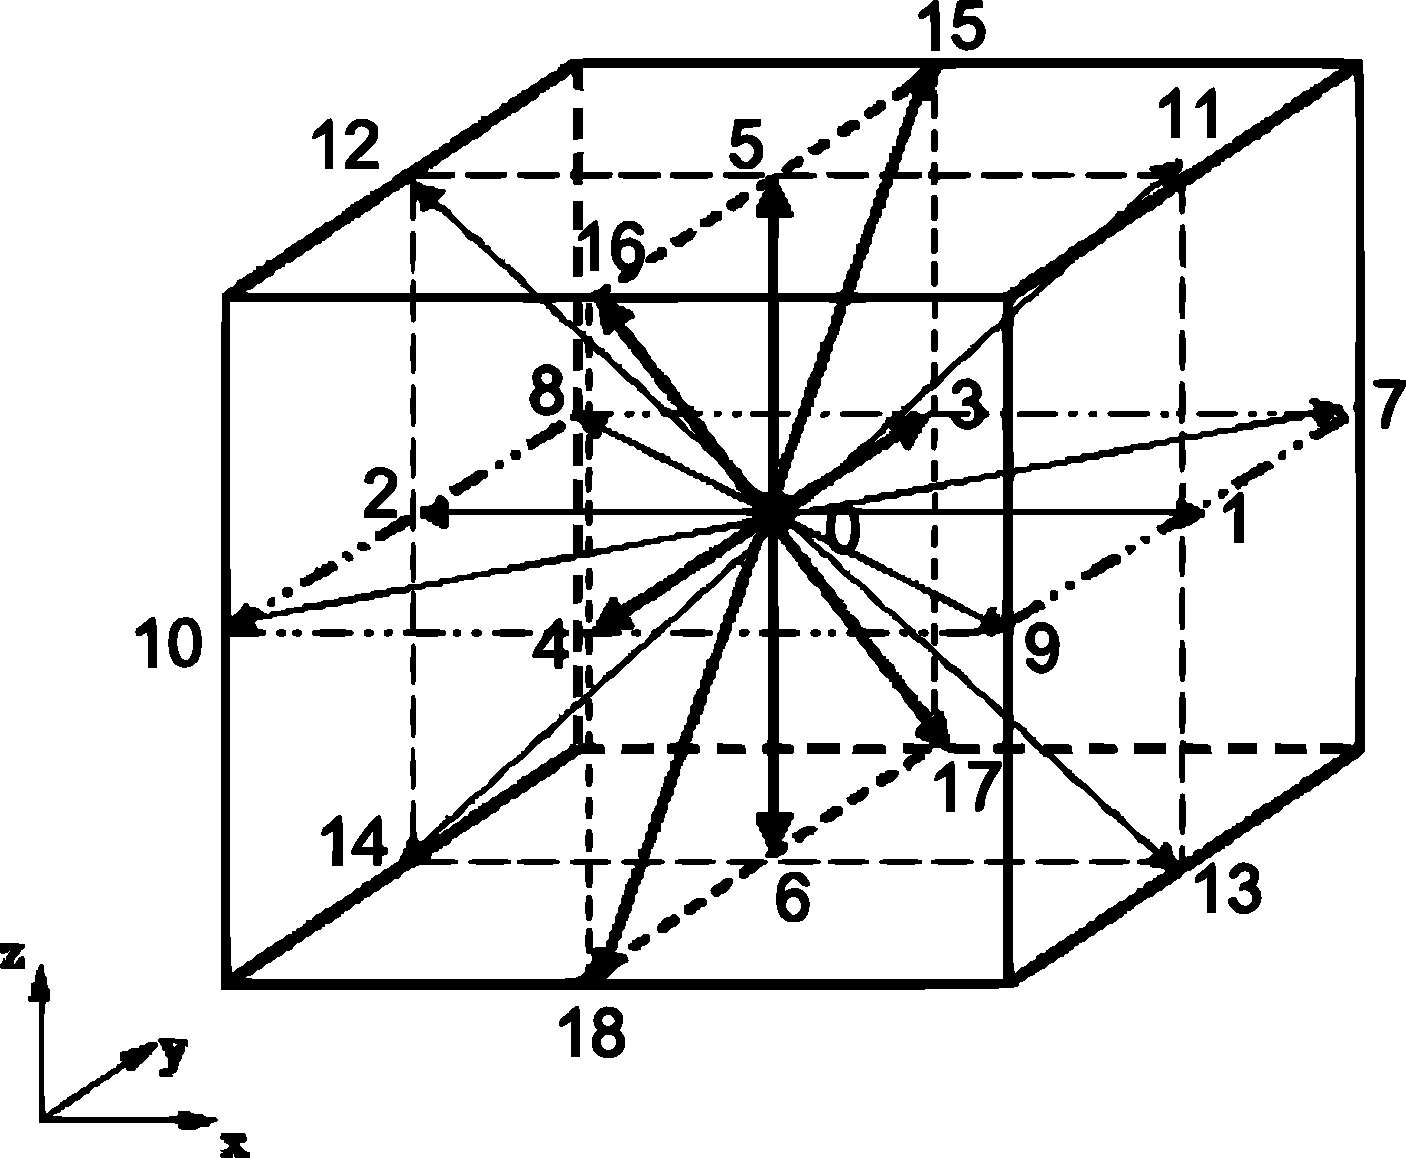
\includegraphics[width=.75\linewidth]{figuras/d3q19.pdf}
  \caption[Esquemático do D3Q19]{Esquemático do modelo D3Q19. Ilustração adaptada do estudo de \citeonline{premnath2013investigation}.}
  \label{fig:d3q19}
\end{figure}

\newpage
\subsection{Múltiplos Tempos de Relaxação}

A Equação (\ref{eq:omega_i}) retrata um operador de colisão com tempo de relaxação único para todas as direções de propagação $i$. Essa abordagem é funcional, porém limitada à estabilidade em baixos números de Reynolds como mostra o estudo de \citeonline{lallemand2000theory}. Para esses tipos de problemas a abordagem de múltiplos tempos de relaxação (MRT)\abreviatura{MRT}{\textit{multiple}-\textit{relaxation}-\textit{time}}, pode ser usada assim como é mostrado nos estudos de \citeonline{viggen2014lattice}.

Seguindo a formulação proposta por \citeonline{d1994generalized}, a formulação de MRT se baseia na troca do parâmetro de único tempo de relaxação $\tau$ por uma matriz \textbf{$\Lambda$} de vários tempos de relaxação. Todavia a matriz \textbf{$\Lambda$} é construída de acordo com uma matriz \textbf{$M$} que projeta as funções de distribuição $f_{i}$ e $f_{i}^{M}$ no espaço dos momentos. De acordo com \citeonline{lallemand2000theory}, a possibilidade desse método ser mais estável é oriunda da capacidade de operar a colisão das células com um tempo de relaxação apropriado para cada um dos vários momentos, projetados a partir das funções de distribuição $f_{i}$ e $f_{i}^{M}$. Em vista do exposto o operador de colisão da Equação (\ref{eq:omega_i}) se transforma em
\begin{equation}
	\Omega_{i} = -\textbf{$\Lambda$}(f_{i} - f_{i}^{M}).
    \label{eq:MRT_1}
\end{equation}
Porém a operação de colisão é realizada no espaço dos momentos. Logo é preciso projetar $f_{i}$ e $f_{i}^{M}$ no espaço dos momentos impondo
\begin{equation}
	m_{i} = \textbf{$M$}f_{i} \text{ e } m_{i}^{M} = \textbf{$M$}f_{i}^{M}.
    \label{eq:MRT_2}
\end{equation}
\citeonline{d1994generalized} propôs, para o caso do modelo D3Q19, uma distribuição de valores para a matriz \textbf{$M$} dada por

% \begin{equation}
%   \tiny {\begin{bmatrix}
% a & b & t \\
% \end{bmatrix}  }
% \end{equation}

\setcounter{MaxMatrixCols}{19}
\begin{equation}
\textbf{$M$} = 
\tiny{\begin{bmatrix}
A &   A &   A &   A &   A &   A &   A &   A &   A &   A &   A &   A &   A &   A &   A &   A &   A &   A &   A \\ 
 B & C & C & C & C & C & C &   D &   D &   D &   D &   D &   D &   D &   D &   D &   D &   D &   D \\ 
  E &  F &  F &  F &  F &  F &  F &   A &   A &   A &   A &   A &   A &   A &   A &   A &   A &   A &   A \\ 
   G &   A &  J &   G &   G &   G &   G &   G &   G &   G &   G &  J &   A &  J &   A &  J &   A &  J &   A \\ 
   G &  F &   K &   G &   G &   G &   G &   G &   G &   G &   G &  J &   A &  J &   A &  J &   A &  J &   A \\ 
   G &   G &   G &   A &  J &   G &   G &   A &  J &  J &   A &   G &   G &   G &   G &   A &  J &  J &   A \\ 
   G &   G &   G &  F &   K &   G &   G &   A &  J &  J &   A &   G &   G &   G &   G &   A &  J &  J &   A \\ 
   G &   G &   G &   G &   G &   A &  J &   A &  J &   A &  J &  J &   A &   A &  J &   G &   G &   G &   G \\ 
   G &   G &   G &   G &   G &  F &   K &   A &  J &   A &  J &  J &   A &   A &  J &   G &   G &   G &   G \\ 
   G &   I &   I &  J &  J &  J &  J &  H &  H &  H &  H &   A &   A &   A &   A &   A &   A &   A &   A \\ 
   G &  F &  F &   I &   I &   I &   I &  H &  H &  H &  H &   A &   A &   A &   A &   A &   A &   A &   A \\ 
   G &   G &   G &   A &   A &  J &  J &   G &   G &   G &   G &  J &  J &  J &  J &   A &   A &   A &   A \\ 
   G &   G &   G &  H &  H &   I &   I &   G &   G &   G &   G &  J &  J &  J &  J &   A &   A &   A &   A \\ 
   G &   G &   G &   G &   G &   G &   G &   G &   G &   G &   G &   G &   G &   G &   G &  J &  J &   A &   A \\ 
   G &   G &   G &   G &   G &   G &   G &   A &   A &  J &  J &   G &   G &   G &   G &   G &   G &   G &   G \\ 
   G &   G &   G &   G &   G &   G &   G &   G &   G &   G &   G &   A &   A &  J &  J &   G &   G &   G &   G \\ 
   G &   G &   G &   G &   G &   G &   G &   G &   G &   G &   G &   A &  J &   A &  J &  J &   A &  J &   A \\ 
   G &   G &   G &   G &   G &   G &   G &   A &  J &  J &   A &   G &   G &   G &   G &  J &   A &   A &  J \\ 
   G &   G &   G &   G &   G &   G &   G &  J &   A &  J &   A &  J &   A &   A &  J &   G &   G &   G &   G \\
\end{bmatrix}},
\end{equation}
sendo $A = 1$, $B = -30$, $C = -11$, $D = 8$, $E = 12$, $F = -4$, $G = 0$, $H = -2$ e $I = 2$.

Considerando que a matriz \textbf{$S$} é dada por
\begin{equation}
	\textbf{$S$} = \textbf{$M$}\textbf{$\Lambda$}\textbf{$M$}^{-1},
    \label{eq:MRT_3}
\end{equation}
o operador de colisão fica
\begin{equation}
	\Omega_{i} = -\textbf{$M$}^{-1}\textbf{$S$}(m_{i} - m_{i}^{M}).
    \label{eq:MRT_4}
\end{equation}
Inserindo a Equação (\ref{eq:MRT_4}) na Equação (\ref{eq:f_i}) fica
\begin{equation}
	f_{i}(\textbf{x} + c_{i}\Delta t, t + \Delta t) = f_{i}(\textbf{x}, t) -\textbf{$M$}^{-1}\textbf{$S$}(m_{i} - m_{i}^{M}).
    \label{eq:MRT_5}
\end{equation}
Vale ressaltar que a operação de propagação, lado esquerdo da Equação (\ref{eq:MRT_5}), ocorre no espaço original da função de distribuição $f_{i}$.


\subsection{Condições de Contorno}

\subsubsection{\textit{Bounceback}}

De acordo com o estudo de \citeonline{viggen2014lattice}, a condição de contorno do tipo \textit{bounceback} tem como objetivo simular uma parede rígida no domínio do LBM, sendo ela do tipo implícita e localizada entre as células. Há dois tipos de \textit{bounceback}: \textit{free-slip}, que simula escorregamento livre do fluido na parede e \textit{no-slip}, que impõe que todas as componentes de velocidade junto à parede sejam nulas. Essa condição força o desenvolvimento da camada limite viscosa junto à parede. Nesse trabalho foi usado a condição do tipo \textit{no-slip}, afim de capturar os efeitos de camada limite viscosa.

A condição de contorno \textit{bounceback} \textit{no-slip} é geralmente implementada na etapa de propagação a partir de uma inversão de funções de distribuição de partículas. A Figura \ref{fig:bounceback} mostra um esquemático de exemplo do processo de funcionamento dessa condição de contorno. Ao cruzar a condição de contorno no tempo seguinte $t + \Delta t$, a célula inverte as funções de distribuição de partículas para o sentido contrário dos vetores que apontam para o \textit{bounceback}.

% \begin{figure}[ht!]
% \centering
%   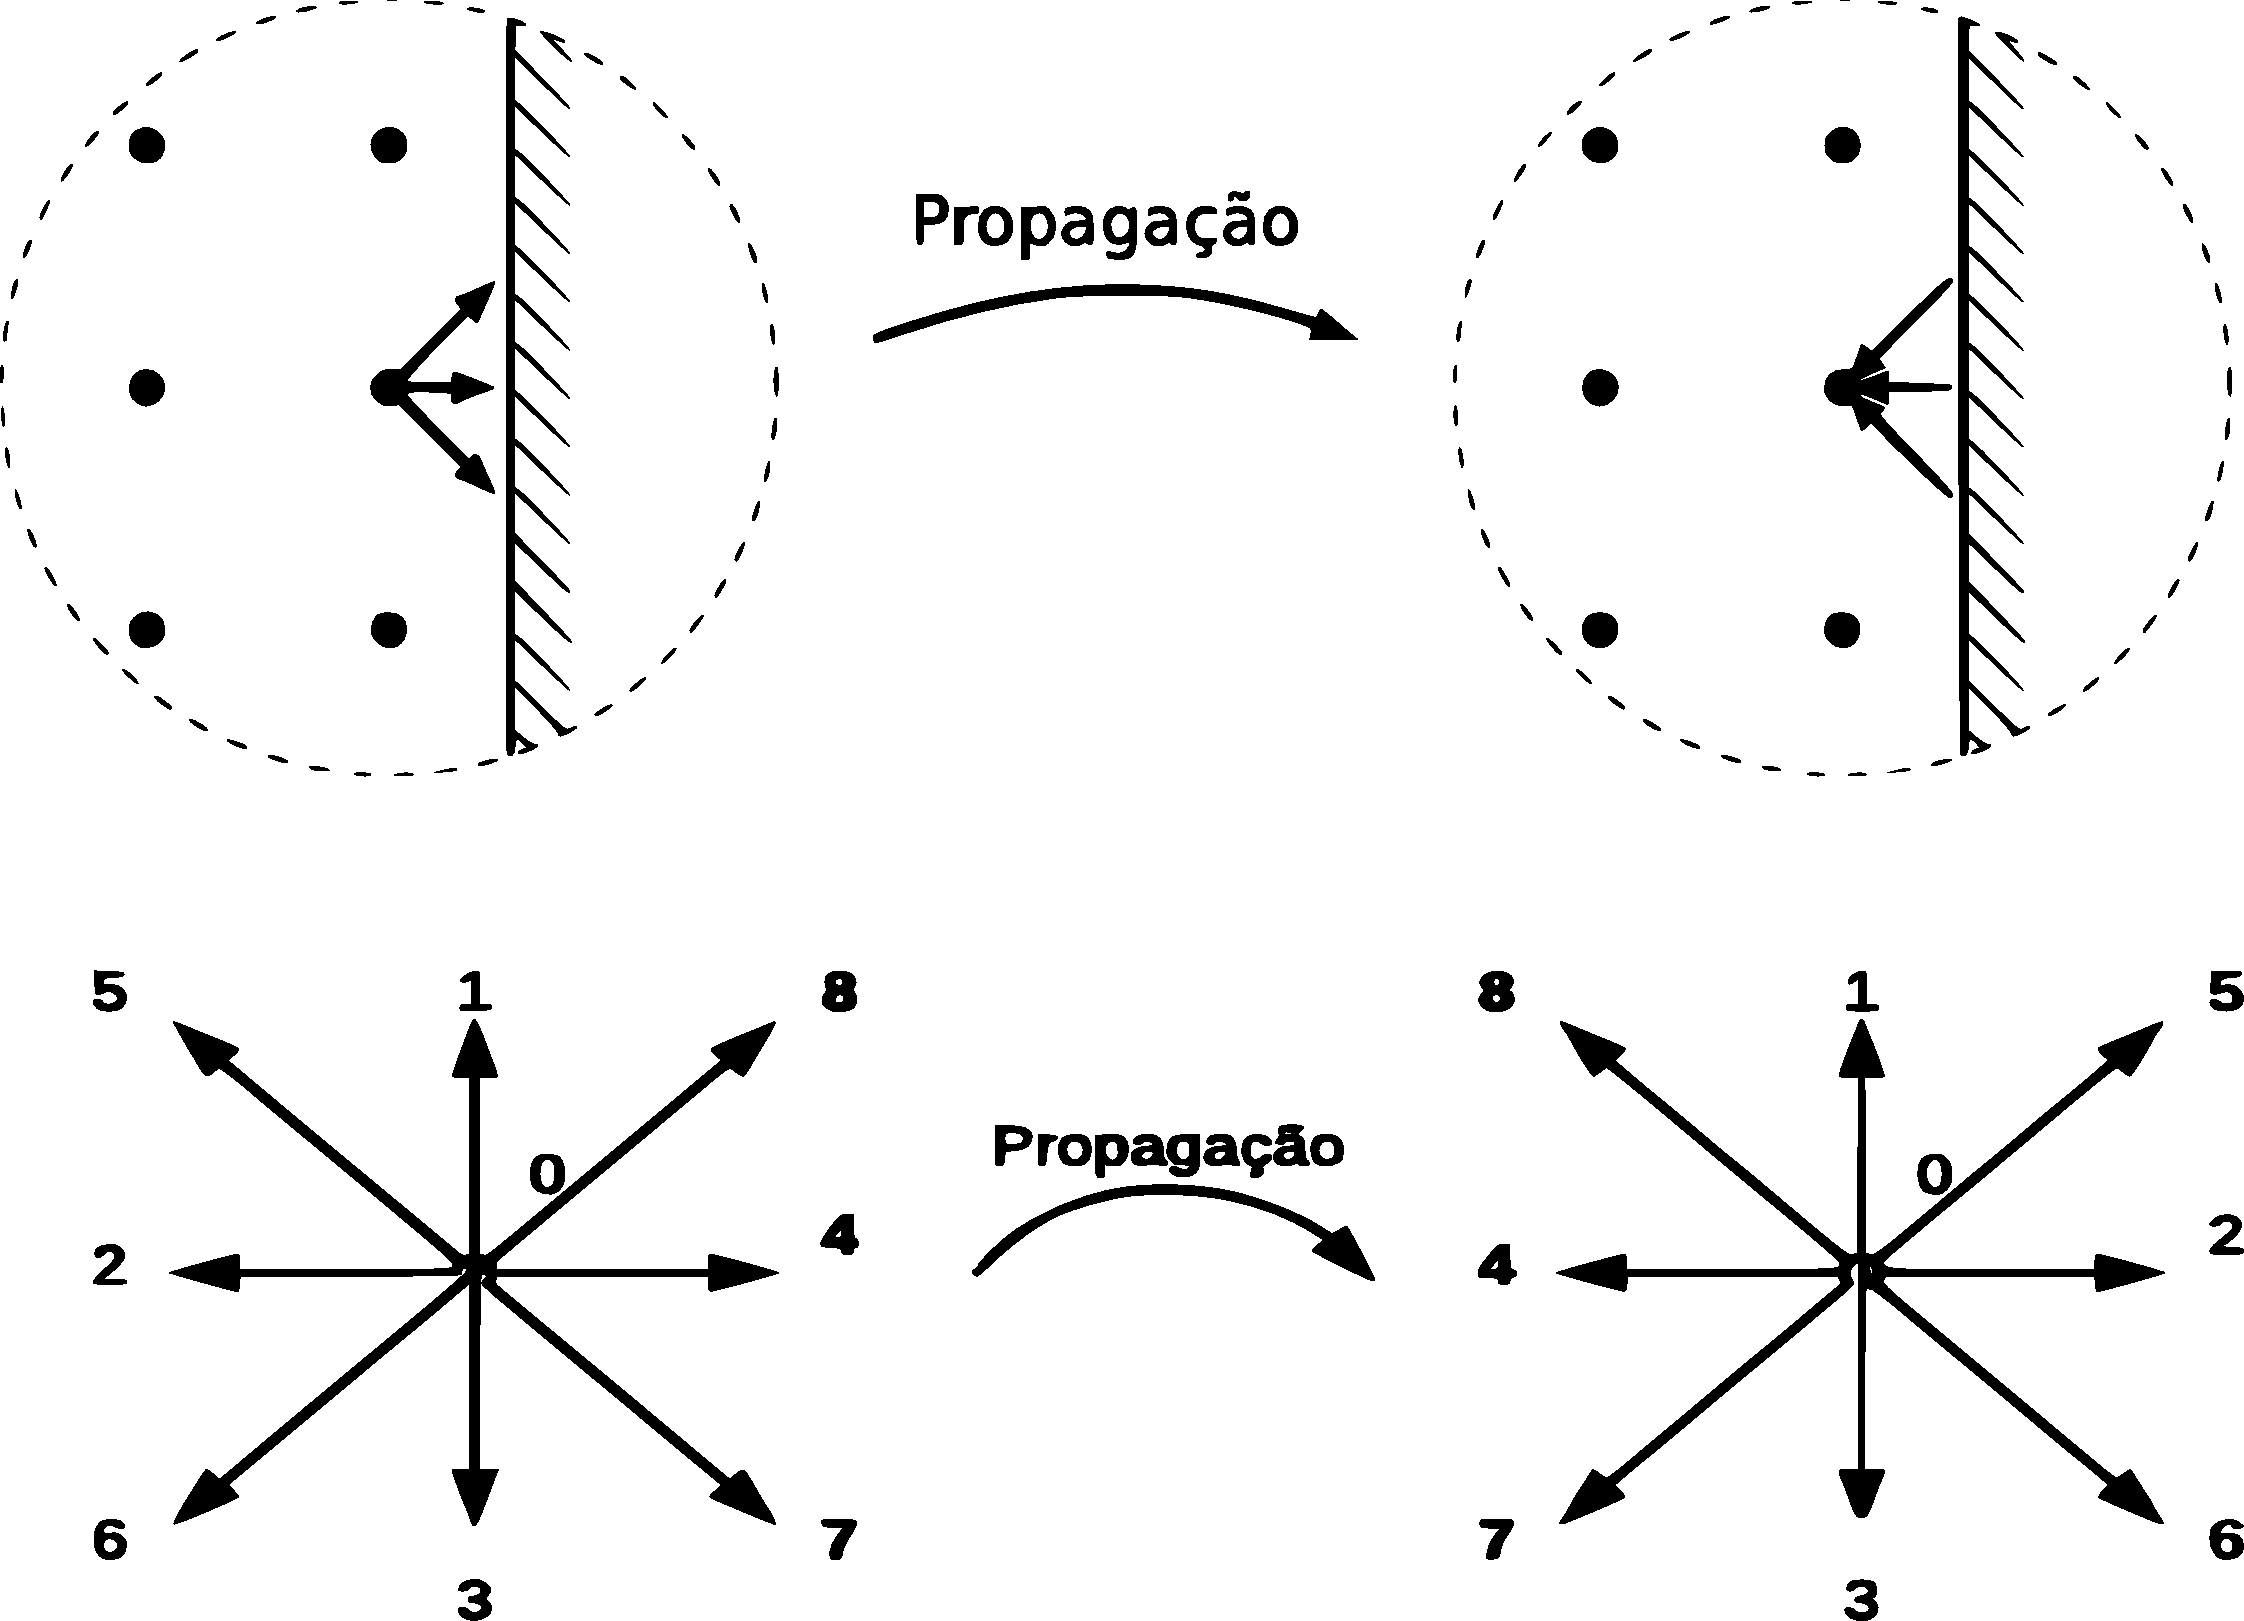
\includegraphics[width=.65\linewidth]{figuras/bounceback.pdf}
  
%   \label{fig:bounceback}
% \end{figure}

\begin{figure}[ht!]
  \centering
  \def\svgwidth{200pt}
  \import{figuras/}{bounceback_2.pdf_tex}
  \caption[Funcionamento do \textit{bounceback} \textit{no-slip}]{Esquemático de exemplo do processo de funcionamento da condição de contorno \textit{bounceback} \textit{no-slip}. Ilustração adaptada do estudo de \citeonline{viggen2014lattice}.}
  \label{fig:bounceback}
\end{figure}

\newpage
Em relação às equações de propagação o processo abordado fica

\begin{gather*}
  f_{6}(\textbf{x}, t + \Delta t) = f_{8}(\textbf{x}, t)\text{,  } f_{8}(\textbf{x}, t + \Delta t) = f_{6}(\textbf{x}, t), \\
  f_{2}(\textbf{x}, t + \Delta t) = f_{4}(\textbf{x}, t)\text{,  } f_{4}(\textbf{x}, t + \Delta t) = f_{2}(\textbf{x}, t) \text{, }\\
  f_{5}(\textbf{x}, t + \Delta t) = f_{7}(\textbf{x}, t)\text{ e } f_{7}(\textbf{x}, t + \Delta t) = f_{5}(\textbf{x}, t).
\label{eq:bounceback}
\end{gather*}

\subsubsection{Condição Anecóica}

Consolidar uma condição do tipo anecóica num método numérico de natureza temporal é um desafio em todos os métodos numéricos. Nesse contexto, considerando a absorção de ondas de pressão, entropia e pulsos de despredimento de vórtices, o trabalho de \citeonline{kam2006non} propõe uma condição de contorno explícita de absorção. Em essência, este método se baseia na adaptação do método das camadas perfeitamente casadas (``\textit{perfectly} \textit{matched} \textit{layers}") para o LBM. A condição de contorno de absorção, \textit{Absorbing} \textit{Boundary} \textit{Condition} (ABC)\abreviatura{ABC}{\textit{Absorbing} \textit{Boundary} \textit{Condition}}, consiste na adição de uma região de amortecimento para que os valores de pressão e velocidade convirjam assintoticamente a valores que caracterizam um fluido em repouso. Nesse sentido, valores alvos para um fluido em resposo de densidade ($\rho_{T}$ $=$ $\rho_{0}$) e velocidade (\textbf{$u_{T}$} $=$ $0$) são usados para calcular uma função de distribuição de amortecimento $f_{i}^{T}$\simbolo{$f_{i}^{T}$}{Função de distribuição de amortecimento}. Essa função de distribuição é definida da mesma forma que $f_{i}^{M}$, porém com os valores alvos de densidade e velocidade, impostos na forma
\begin{equation}
  f_{i}^{T} = \rho_{0}\varepsilon_{i}.
  \label{eq:f_alvo}
\end{equation}
Como essa técnica é explícita, o operador de colisão $\Omega_{i}$ da Equação (\ref{eq:omega_i}) é adaptado e recebe um novo termo fonte, tal que
\begin{equation}
  \Omega_{i} = -\frac{1}{\tau}(f_{i} - f_{i}^{M}) - \sigma(f_{i}^{M} - f_{i}^{T}),
  \label{eq:omega_i_abc}
\end{equation}
sendo $\sigma$ $=$ $\sigma_{T}(\delta/D)^{2}$ o coeficiente de absorção, $\sigma_{T}$ uma constante com valor de $0,3$, $\delta$ é a distância medida do começo da região de contorno no sentido da convergência assintótica e $D$ é o tamanho total da região de contorno no sentido da convergência assintótica assim como ilustra a Figura \ref{fig:abc}.

\begin{figure}[ht!]
\centering
  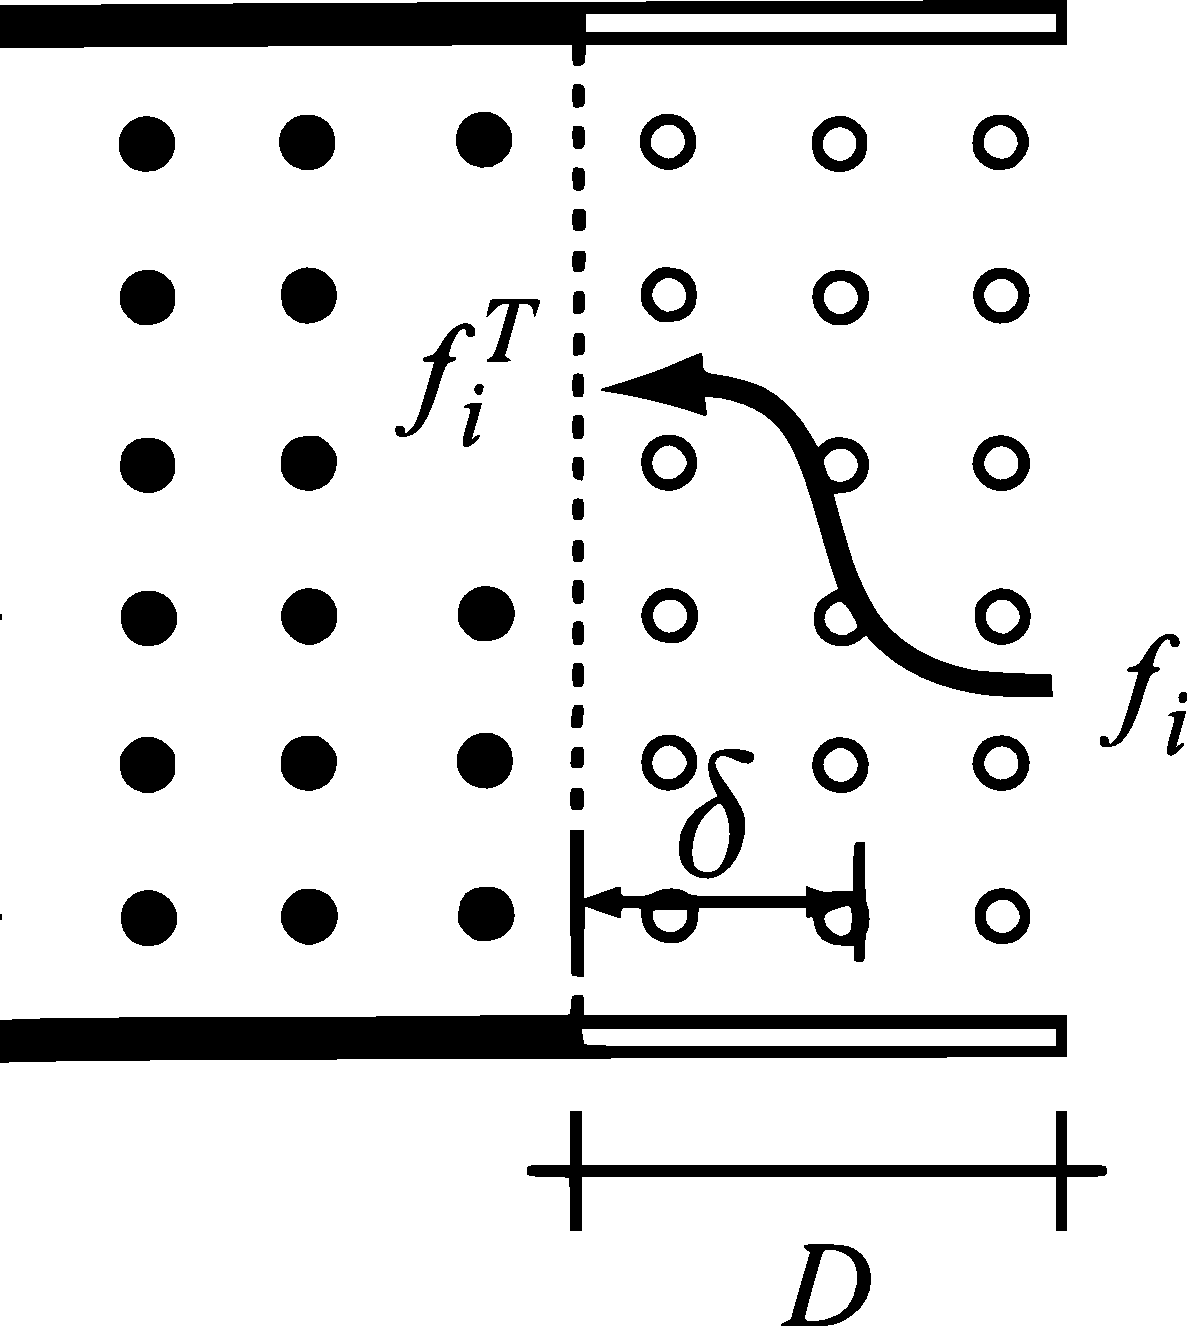
\includegraphics[width=.3\linewidth]{figuras/abc.pdf}
  \caption[Funcionamento da condição de contorno anecóica]{Esquemático de exemplo do processo de funcionamento da condição de contorno anecóica. Ilustração adaptada do estudo de \citeonline{da2008numerical}.}
  \label{fig:abc}
\end{figure}

O operador de colisão da Equação (\ref{eq:omega_i_abc}) funciona bem para o modelo SRT, porém como nesse estudo será usado o modelo MRT, algumas adaptações precisam ser realizadas, pois a operação de colisão ocorre no espaço dos momentos nesse modelo. Assim como é feito nas Equações (\ref{eq:MRT_2}) deve-se aplicar o mesmo procedimento na função de distribuição $f_{i}^{T}$ originando o termo $m_{i}^{T}$. Além disso é preciso inserir esse termo no operador de colisão da Equação (\ref{eq:MRT_4}) resultando em 

\begin{equation}
  \Omega_{i} = -\textbf{$M$}^{-1}\textbf{$S$}(m_{i} - m_{i}^{M}) - 
  \sigma\textbf{$M$}^{-1}\textbf{$S$}(m_{i}^{M} - m_{i}^{T}).
  \label{eq:abc_mrt_2}
\end{equation}

Simplificando, a Equação (\ref{eq:abc_mrt_2}) fica
\begin{equation}
  \Omega_{i} = -\textbf{$M$}^{-1}\textbf{$S$}[m_{i} - m_{i}^{M}(\sigma - 1) - m_{i}^{T}].
  \label{eq:abc_mrt_3}
\end{equation}

Adicionando esse termo na Equação geral (\ref{eq:f_i}) do LBM, o resultado é a equação
\begin{equation}
  f_{i}(\textbf{x} + c_{i}\Delta t, t + \Delta t) = f_{i}(\textbf{x}, t) -\textbf{$M$}^{-1}\textbf{$S$}[m_{i} - m_{i}^{M}(\sigma - 1) - m_{i}^{T}].
  \label{eq:abc_mrt_4}  
\end{equation}

A Equação (\ref{eq:abc_mrt_4}) equivale a Equação (\ref{eq:f_i}) porém com um termo fonte adicional representando a camada anecóica. Vale ressaltar que esse termo fonte é nulo no domínio fluidodinamico e diferente de zero na camada absorvente.

\section{Palabos}

O \textit{software} livre Palabos é um projeto feito na linguagem C++ no paradígma computacional de orientação a objetos, resultado da colaboração entre indústria e academia, focando produzir uma ferramenta de simulação computacional robusta, rápida e confiável. Junto com esse pacote computacional há implementados modelos numéricos de publicações e \textit{benchmarks} da litetura, como mostra os estudos de \citeonline{lattice_1}, \citeonline{lattice_2}, \citeonline{lattice_3}, \citeonline{lattice_4} e \citeonline{lattice_5}. 

As funcionalidades do \textit{software} Palabos usadas nesse trabalho são: modelo base (MRT); condição de contorno (\textit{bounceback} \textit{no-slip}); \textit{grid} (D3Q19); paralelismo (MPI em vários processadores); dados de saída (ASCII, GIF e VTK para visualização no \textit{software} \citeonline{paraview}).

Mesmo com várias funcionalidades citadas, o \textit{software} Palabos precisa ter outras outras funcionalidades implementadas para que possa atender o escopo desse trabalho. Para atender esse requisito, o projeto \citeonline{palabos_acoustic} foi criado como uma versão do Palabos que contém todos os modelos e implementações desenvolvidas nesse trabalho. As funcionalidades desenvolvidas nesse trabalho são: condição de contorno anecóica de \citeonline{kam2006non} para BGK D2Q9 e MRT D2Q9 e D3Q19; condição de contorno para excitação do duto com \textit{sweep} de acordo com o estudo de \citeonline{da2009sound} ou excitação por soma de harmônicos.


\section{Modelo Numérico}
\label{sec:modelo_numerico}

Com os arquivos de compilação e execução corretamente configurados, pode-se modelar numericamente o problema. A Figura \ref{fig:modelo} representa a vista do corte lateral do modelo numérico tridimensional com o eixo de coordenadas localizado no ponto $(\frac{\textbf{Nx}}{2}, 0, 0)$. Para a definição do domínio foi utilizado uma abordagem paramétrica, ou seja, o raio externo do duto $a$ $=$ $20$ células foi a unidade de medida para as dimensões. As dimensões \textbf{Nx} e \textbf{Ny} são iguais e possuem $20a$ de comprimento (razão de aspecto não mantida no esquema para economia do espaço em folha). A dimensão \textbf{Nz} possui 79,5$a$ de comprimento e foi baseado no estudo de \citeonline{da2009sound}, que justifica a distância da saída do duto até a parede para capturar corretamente os efeitos de inércia e elasticidade produzidos pelo fluido estagnante ao redor do duto. Todo espaço de fluido do domínio foi preenchido em cada célula com frequência de relaxação $\frac{1}{\tau}$ $=$ $1,99$, $\rho$ $=$ $\rho_{0}$ $=$ $1$ e as velocidades para todos os sentidos $u_{x}$ $=$ $u_{y}$ $=$ $u_{z}$ $=$ $0$. As bordas do duto foram preenchidas com condição anecóica de espessura igual 1,5$a$ células. Além disso vale ressaltar que, considerando a viscosidade do ar como $15,11 \dot 10^{-6}$ e números de Reynolds e Mach máximos do modelo numérico iguais a 5514,82 e 0,2 respectivamente, o tamanho de uma célula ($\Delta x$) equivale a $3,036 \dot 10^{-5}$ metros. Nesse sentido, valor do raio $a$ do duto é igual a 0,61 milímetros.

Com relação ao duto, o mesmo possui o tamanho \textbf{L} $=$ $18a$ e é delimitado pela condição de contorno \textit{bounceback} \textit{no-slip}. O diâmetro externo mede $2a$ e parede com expessura de 0,1$a$. No começo do duto há uma condição anecóica com espessura igual a 1,5$a$, que é responsável pela absorção da onda refletida na abertura do duto. Ao lado da condição anecóica há uma condição de contorno de excitação do duto com espessura de 0,05$a$, responsável por excitar os modos axiais e impor escoamento.    

% \begin{figure}[ht!]
%   \centering
%   \def\svgwidth{400pt}
%   \import{figuras/}{modelo_numerico.pdf_tex}
%   \caption[Esquemático do modelo numérico]{Esquemático do modelo numérico: vista do corte lateral do modelo em 3D.}
%   \label{fig:modelo}
% \end{figure}

\begin{figure}[ht!]
\centering
  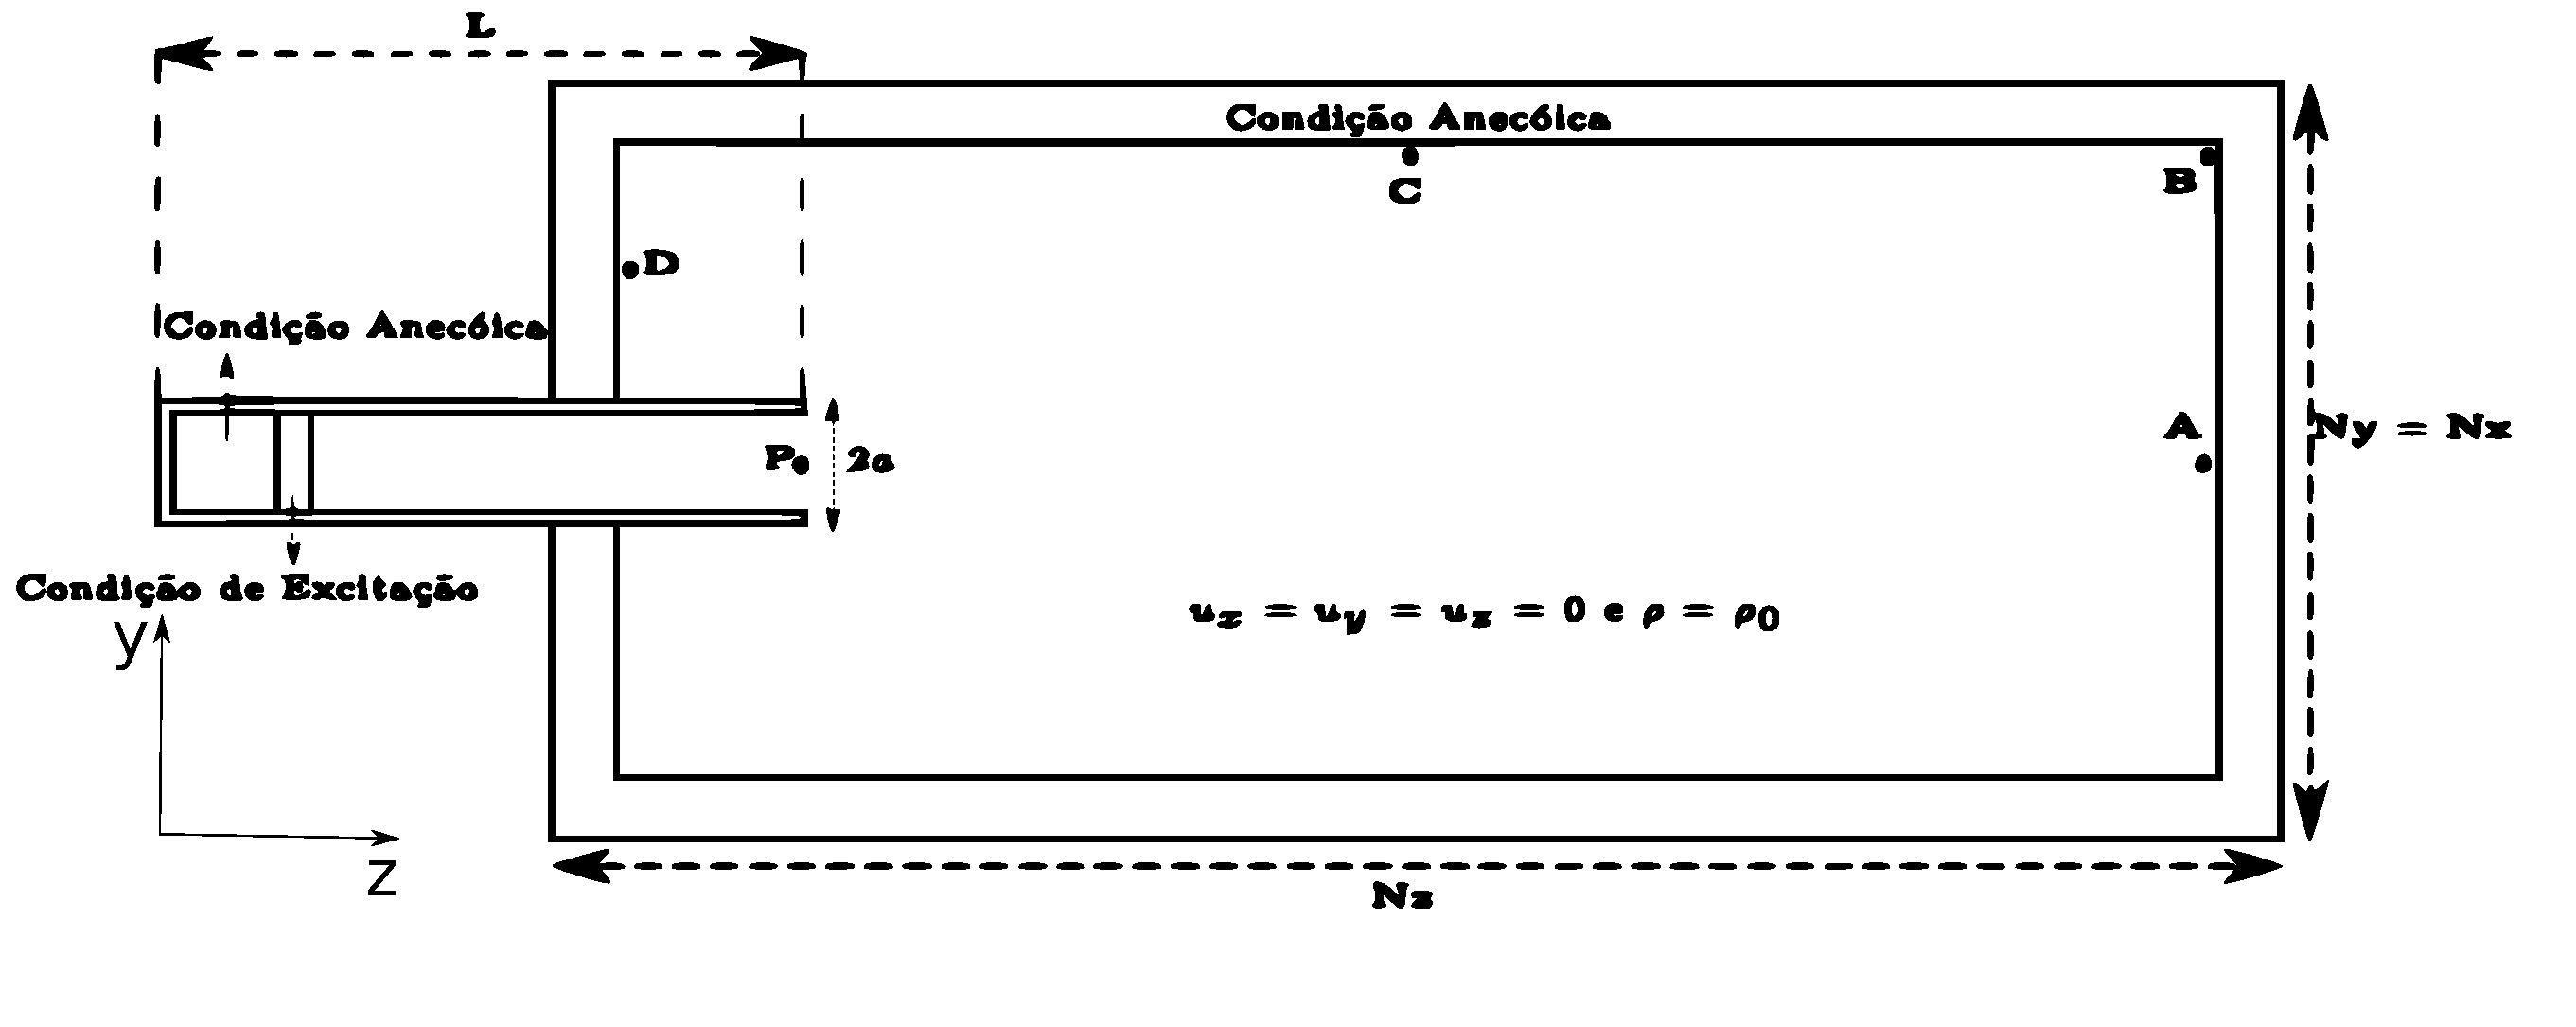
\includegraphics[width=1.\linewidth]{figuras/modelo_numerico_3.pdf}
  \caption[Esquemático do modelo numérico]{Esquemático do modelo numérico: vista do corte lateral do modelo em 3D.}
  \label{fig:modelo}
\end{figure}


Focando propiciar energia suficiente nos modos axiais com onda plana, a condição de excitação foi desenvolvida através de uma soma de ondas estacionárias, na faixa de frequência $0$ $<$ $ka$ $\leq$ 2,5. Dessa forma, os valores de densidade e velocidade dessa região foram mudados em cada incremento de tempo da seguinte forma:
\begin{itemize}
  \item regime transiente ($0 \leq t < t_{transiente}$):
  \begin{gather*}
    \rho(t) = \rho_{0};% + A\sum_{n=1}^{N} sin\bigg(\frac{nka_{max}c_{s}t}{Na}\bigg);
    \\ u_{z}(t) = Mc_{s};    
    \\ u_{y}(t) = 0;
    \\ u_{x}(t) = 0.
  \label{eq:transiente}
  \end{gather*}

  \item regime estacionário ($t_{transiente} \leq t \leq t_{total} - t_{propagada}$):
  \begin{gather*}
    \rho(t) = \rho_{0} + A\sum_{n=1}^{N} sin\bigg(\frac{nka_{max}c_{s}t}{Na}\bigg);
    \\ u_{z}(t) = Mc_{s} + \frac{Ac_{s}}{\rho_{0}}\sum_{n=1}^{N} sin\bigg(\frac{nka_{max}c_{s}t}{Na}\bigg);    
    \\ u_{y}(t) = 0;
    \\ u_{x}(t) = 0.
  \label{eq:estacionario}
  \end{gather*}
\end{itemize}
tal que $ka_{max} =$ 2,5, $N$ é o número total de componentes harmônicos dentro do intervalo $0$ $<$ $ka$ $\leq$ 2,5, $n$ é a $n$-ésima componente harmônica dentro desse intervalo. $t_{transiente}$ é é o número de incrementos de tempo necessessários para atingir o regime estacionário. Este valor se baseou no estudo de \citeonline{shi2013lattice} na forma $t_{transiente} =  2\textbf{Nz}/Mc_{s}$, $t_{propagada}$ é definido como $t_{propagada} = \textbf{Nz}/c_{s}$ e é o tempo que a onda demora para percorrer o domínio completo na direção axial do duto, $t_{total} = t_{transiente} + t_{propagada} + 12000$ é o tempo total da simulação e $A$ é definida em termos de densidade. Esta é calculada por
\begin{equation}
  A = \frac{2 \cdot 10^{-5} \cdot 10^{\text{NPS}/20}}{c^{*}\rho^{*}_{0}c_{s}},
\end{equation}
tal que $c^{*} = 343$ $m/s$ é a velocidade do som em unidades físicas, $\rho^{*}_{0} =$ 1,22 $kg/m^{3}$ é a densidade física do ar em unidades físicas e NPS é o nível de pressão sonora no valor de 80 dB.

\subsection{Verificação da Condição Anecóica}

No intuito de avaliar a condição anecóica nas fronteiras do domínio através do cálculo e análise do coeficiente de reflexão, os pontos $\textbf{A}$, $\textbf{B}$, $\textbf{C}$ e $\textbf{D}$ representados na Figura \ref{fig:modelo} são utilizados para medição de pressão e velocidade de partícula acústica na fronteira com a terminação anecóica. O local dos pontos é definido pelas seguintes coordenadas:

\begin{itemize}
  \item ponto $\textbf{A}$: $(\frac{\textbf{Nx}}{2}, \frac{\textbf{Ny}}{2}, \textbf{Nz} - 31)$;
  \item ponto $\textbf{B}$: $(\frac{\textbf{Nx}}{2}, \textbf{Ny} - 31, \textbf{Nz} - 31)$;
  \item ponto $\textbf{C}$: $(\frac{\textbf{Nx}}{2}, \textbf{Ny} - 31, \frac{\textbf{Nz}}{2})$;
   \item ponto $\textbf{D}$: $(\frac{\textbf{Nx}}{2}, \frac{3\textbf{Ny}}{4}, 12a + 31)$.
\end{itemize}
 
Já o ponto $\textbf{P}$ representa a média espacial, feita no plano transversal do duto, dos valores de pressão e velocidade de partícula na terminação. Essas médias espaciais são extraídas e calculadas ao longo do tempo para se obter os parâmetros de caracterização da acústica interna do duto: coeficiente de reflexão $R_{r}$ e coeficiente de correção da terminação $l/a$.

Para a execução da simulação numérica foi escolhido um \textit{hardware} com as seguintes características:

\begin{itemize}
  \item arquitetura: x86\_64;
  \item CPU(s): 8;
  \item modelo do processador: Intel(R) Xeon(R) CPU E5620 @2.40GHz;
  \item memória RAM: 139 GB.
\end{itemize}

%\newcommand{\MyNumberA}{30}

%\newcommand{\MyNumberB}{60}

%\MyNumberB

%\numexpr (\MyNumberA + 2* \MyNumberN)/3 \relax
%\the\numexpr (\MyNumberA * \MyNumberB)

\section{Pós-processamento}

Com os arquivos de dados temporais dos pontos $\textbf{A}$, $\textbf{B}$, $\textbf{C}$, $\textbf{D}$ e da média espacial $\textbf{P}$ salvos em disco rígido, um \textit{script} de pós-processamento da plataforma \citeonline{matlab}/\citeonline{octave} é executado. Os seguintes procedimentos são realizados no \textit{script}:

\begin{enumerate}
  \item os vetores temporais de pressão e velocidade no eixo axial são obtidos através da leitura de arquivos \textbf{.dat};
  \item uma janela Hanning na forma
  \begin{equation}
    w(n) = sin^{2}\bigg(\frac{\pi n}{N - 1} \bigg),  
  \end{equation}
  tal que $N$ é o tamanho da janela e $n$ é a posição do vetor unidimensional é definida e usada para multiplar os sinais de velocidade e pressão no domínio do tempo;

  \item a transformada discreta de Fourier, utilizando o algorítmo de transformada rápida, \textit{Fast} \textit{Fourier} \textit{Transform} (FFT)\abreviatura{FFT}{\textit{Fast} \textit{Fourier} \textit{Transform}}, foi utilizada para transformar os históricos temporais de pressão e velocidade de partícula para o domínio da frequência;

  \item a impedância de radiação $Z_{r}$ é calculada através da divisão entre os vetores de pressões por de velocidades no domínio da frequência da seguinte forma:
  \begin{equation}
    Z_{r} = \frac{p(f)}{u_{z}(f)};
  \end{equation}

  \item a magnitude do coeficiente de reflexão $|R_{r}|$ é calculado de acordo com a Equação (\ref{eq:R});
  \item o coeficiente de correção da terminação $l/a$ é calculado de acordo com a Equação (\ref{eq:l});
 \end{enumerate}

 Para minimizar os efeitos não lineares de ondas evanescentes na terminação do duto e o efeito da espessura do duto (equivalente a duas células), um fator de correção $c = - 0,2367$ é adicionado na parte real do coeficiente de correção da terminação $l/a$.

Para fins de comparação dos resultados obtidos nesse estudo com resultados da literatura foi usado o coeficiente de correlação de Pearson na forma
\begin{equation}
  r = \Bigg|\frac{\sum_{j=1}^{J} (x_{j} - \overline{x})(y_{j} - \overline{y})}{\sqrt{\sum_{j=1}^{J} (x_{j} - \overline{x})^{2}} \sqrt{\sum_{j=1}^{J} (y_{j} - \overline{y})^{2}}}\Bigg| \times 100,
  \label{eq:correlacao}
\end{equation}
tal que $r$ é um percentual, sendo que quanto maior o valor mais correlacionado o resultado do modelo numérico estará com modelos da literatura. $J$ é o número total de pontos, $x_{j}$ e $y_{j}$ são valores de dois conjuntos de pontos na posição $j$ a serem comparados e $\overline{x}$ e $\overline{y}$ são as médias definidas nas formas
\begin{equation}
  \overline{x} = \frac{\sum_{j=1}^{J} x_{j}}{J} \text{ e }
\end{equation}
\begin{equation}
  \overline{y} = \frac{\sum_{j=1}^{J} y_{j}}{J}. 
\end{equation}

\section{Integral de Energia de Howe}

Em vista da literatura vigente, fenômenos aeroacústicos envolvendo baixos números de Reynolds são muito peculiares pelo fato do campo acústico ser alterado pela transferência de energia cinética vorticial em energia acústica e vice-versa. Para investigar tal fenomenologia, a integral de energia de Howe apresenta-se como uma ferramenta apelativa.

De acordo com o estudo de \citeonline{howe1984absorption} a integral de energia de Howe é uma descrição formal da transferência da energia cinética vorticial para o campo acústico e vice-versa num contexto de baixos números de Mach ($M << 1$) e escoamentos isoentrópicos. Tal formulação é expressa por 

\begin{equation}
  <P> = -\rho_{0}\int_{V}< \boldsymbol{\xi} > dV,
  \label{eq:integral_howe_1}
\end{equation}
tal que $<P>$\simbolo{$<P>$}{Potência acústica} é a potência acústica média ao longo de um ciclo de oscilação em torno de um volume $V$, $\rho_{0}$ é a densidade média do fluido e $\boldsymbol{\xi}$\simbolo{$\boldsymbol{\xi}$}{Potência acústica instantânea por unidade de volume} é a potência acústica instantânea por unidade de volume gerada a partir da energia cinética vorticial. Potência acústica instantânea por unidade de volume é expressa por 
\begin{equation}
  \boldsymbol{\xi} = \textbf{u}_{ac} \cdot ( \boldsymbol{\omega} \times \textbf{u}),
  \label{eq:integral_howe_2}
\end{equation}
tal que $\textbf{u}_{ac}$\simbolo{$\textbf{u}_{ac}$}{Velocidade de partícula} é a velocidade de partícula, $\boldsymbol{\omega}$\simbolo{$\boldsymbol{\omega}$}{Rotacional do escoamento} é o rotacional do escoamento e $\textbf{u}$ é a velocidade do escoamento. Para o uso da integral de energia de Howe, foi implementada uma classe dentro do núcleo do \textit{software} Palabos, sendo ativada e instanciada no final de cada simulação do modelo numérico.     